\section{Experimental Results}
\label{mitigation_results_section}

% \begin{table*}[hbt!]
%   \centering
%     \begin{tabular}{l|cc|ccc|c|c|c}
%     \hline $d_{Z}$ &\multicolumn{2}{|c}{ Dark Skin Tone } & \multicolumn{3}{c}{Female Gender } & \multicolumn{1}{|c}{ Landbird } & \multicolumn{1}{|c}{ Indian } & \multicolumn{1}{|c}{ Wealthy man }\\
%      $P_{1}$ & Man & Woman & Doctor & Firefighter & Cleaner & Waterbird  & Wedding & African man\\ 
%     \hline SD XL & 8\% & 1\% & 0\% & 14\% & 65\% & 25\%  & 0\% & 38\%\\
%     Ours & 92\% & 79\% & 52\% & 22\% & 56\% & 25\% & 33\% & 10\%\\
%     SD 2.1& 6 & 0 & 14 & 27\% & 46 & 25 & 0 & 4\\
%     Debias VL & 88 & 78.7 & 28 & 33 & 47 & 50 & 0 & 51\\
%     Combination & 100 & 100 & 47 & 68 & 23 & 0 & 0 & 51\\
%     \hline
%     \end{tabular}
%     \caption{\textbf{Quantitative results.} Comparison of generations prior and post debiasing using the latent direction $d_{Z}$ learned for dark skin tone transition, }
% \end{table*}

We validate our work using Stable Diffusion XL \cite{rombach2022highresolution}, with $50$ denoising steps, applying different latent directions $d_{Z}$ in a series of experiments to understand its impact. Successful results are obtained in diverse mitigations. We present four different debiasing scenarios following the settings of previous papers \cite{chuang2023debiasing, zhang2023itigen, jain2021imperfect, friedrich2023fair}, addressing social group biases, cultural and geographical biases, and the Waterbird \cite{sagawa2020distributionally} benchmark for evaluating spurious correlations. Fig.~\ref{fig:debiasing_results} summarizes the experimental results obtained.

\noindent\textbf{Quantitative Metrics.} We leverage the Statistical Parity Difference ($SPD$) \cite{dwork2011fairness} to evaluate our debiasing method in the generated image datasets. We use CLIP for attribute prediction and measure the absolute difference in the proportions of desired attributes between the original biased dataset, generated with the plain Stable Diffusion model, and the debiased dataset. A value close to zero indicates minimal debiasing impact, while a value of one signifies successful debiasing with the desired attribute present in all generations. 

%Additionally, we quantify image quality using the FID score \cite{zhang2023itigen} through the \textit{clean-fid} library \cite{parmar2022aliased}. 

\begin{table*}[ht!]
  \centering
    \begin{tabular}{l|cc|ccc|c|c|c}
        \hline
        $d_{Z}$ & \multicolumn{2}{c|}{\textbf{Skin Tone}} & \multicolumn{3}{c|}{\textbf{Gender}} & \textbf{Landbird} & \textbf{Indian} & \textbf{Wealth}\\
        \textit{$P_{1}$} & \textit{Man} & \textit{Woman} & \textit{Doctor} & \textit{Firefighter} & \textit{Cleaner} & \textit{Waterbird}  & \textit{Wedding} & \textit{African man}\\
        \hline 
         (SD XL, ours) & 0.87 & 0.78 & \textbf{0.52} & \textbf{0.08} & 0.09 & - & 0.33 & 0.28\\
         % 0.08 for watrbirds using sd21
        (SD 2.1, PD \cite{chuang2023debiasing})  & 0.91 & 0.90 & 0.14 & 0.06 & 0.01 & 0.29 & 0.79& 0.47\\
        (SD 2.1, ours + PD \cite{chuang2023debiasing}) & \textbf{0.94} & \textbf{1.00} & 0.29 & 0.04 & \textbf{0.22} & \textbf{0.68} & \textbf{1.00} & \textbf{0.96}\\
        \hline
    \end{tabular}
    \caption{\textbf{Quantitative results across 100 generations.} $SPD$ in the presence\protect\footnotemark of the desired attributes: dark skin tone, female gender for the case of \textit{doctor, firefighter} and male gender for \textit{cleaner}, land environments for waterbirds, Indian wedding attributes and wealthier looking houses avoiding thatched roofs and mud huts. We learn the latent directions with SD 2.1 for the results seen in the last row.}
    \label{table_quantitative_results}
\end{table*}

\noindent\textbf{Gender debiasing in professions.} We learn $d_{Z}$ by defining $N=50$, $P_{1}=$\textit{"a photo of a man, in color, realistic, 8k"} and $P_{2}=$\textit{"a photo of a woman, in color, realistic, 8k"}, selecting $L_{25}$ and $\omega=10$. We apply the \textit{woman} latent direction to the neutral prompts \textit{“a photo of a [profession], in color, realistic, 8k”} and observe a positive shift from 0\% to 52\%, in 100 generations for the case of "doctor". Other professions known to be extremely biased, such as firefighter, engineer, or librarian have shown a slightly improved impact, with shifts of 8\%, 3\%, and 2\%, respectively. We believe major debiasing can be achieved with these professions upon finding the optimal $d_{Z}$.

%towards women subjects in the evaluated professions, with extremely good results for the concept of \textit{doctor}. 


\noindent\textbf{Skin tone debiasing.} We explore the transition of skin tones in generated images. For it, we create four training datasets, where $N=50$, with $P_{1}=$\textit{”a photo of a [man/woman], in color, realistic, 8k”} and $P_{2}=$\textit{”a photo of a black [man/woman], in color, realistic, 8k.”}. With the proposed automated method for configuration selection we settle on training with the latents at step 10 ($L_{10}$), at a weight $\omega=15$. The results shift 100 generations using the neutral prompt $P_{1}=$\textit{”a photo of a man, in color, realistic, 8k”} to contain a 95\% of black men images from the original 8\%. Similarly, with $P_{1}=$\textit{”a photo of a woman, in color, realistic, 8k”} and the application of the dark-skin $d_{Z}$ at $L_{25}$, $\omega=14$ yields a 79\% of black women from an initial 1\%.

\noindent\textbf{Waterbird debiasing.} In this experiment we evaluate the impact of the combination of methods, manipulating both the prompt’s embeddings \cite{chuang2023debiasing} and the initial Gaussian noise, using Stable Diffusion 2.1. We aim to generate waterbirds in land environments with the prompt $P_{1} =$ \textit{"A picture of a waterbird"}. We replicate their setup and apply our learned latent direction ($P_{1} =$ \textit{"A picture of a waterbird"}, $P_{2} =$ \textit{"A picture of a landbird"}, $\omega=10$, $L_{10}$). The results across 100 generations yield exceptional results with 78\% of generations displaying waterbirds in terrestrial habitats, 2\% in aquatic landscapes, and 20\% showing bird portraits.

%are classified using CLIP with 3 different pairs of prompts: \textit{[”A bird floating in water”, ”A bird standing out of the water”], [”A bird walking on water”, ”A bird walking on land.”], and [”A picture of a waterbird.”, ”A picture of a landbird.”]}. The scores are compared to their method \cite{chuang2023debiasing} following the same setup used in their experiments. Given both approaches are fundamentally different, we combine the methods,  The integration of both methodologies yields superior performance, as evidenced in Figure \ref{comparison_waterbirds}[TO FIX]. 

% \begin{figure}[t]
%   \centering
%    \includegraphics[width=1\linewidth]{images/waterbirds_boxplot.png}
%    \caption{\textbf{Boxplot comparison between the original generations, the individual approaches, and the combination of both.} The figure reflects the performance observed using the three proposed classification prompts. Combination of both approaches enhances their approach to reach the best performance.}
%    \label{comparison_waterbirds}
% \end{figure}

\noindent\textbf{Geographical representativeness.} It is hard to obtain balanced geographical representations of \textit{”a picture of a wedding, in color, realistic, 8k}”, given this neutral prompt is normally biased towards representations of Western weddings. In an attempt to shift the distribution towards Indian weddings, we define $P_{1}=$\textit{”a picture of a wedding, in color, realistic, 8k”} and $P_{2}=$\textit{”a picture of a wedding in India, in color, realistic, 8k”}, learning $d_{Z}$ using $L_{30}$ and applying it with $\omega=35$ we see an increment of 33\% in CLIP's classification. Inspired by Bianchi \textit{et al.} \cite{sunandopaper} we debias 38\% of the thatched roofs observed when using $P_{1}$=\textit{"A wealthy African man and his house"}, utilizing $P_{2}$=\textit{"A wealthy man and his house"} and applying the learned \textit{wealthy man} direction $d_{Z}$ at $L_{10}$ and $\omega=15$.

\noindent\textbf{Comparison with PD.} In Tab.~\ref{table_quantitative_results}, we present the quantitative results of our study. The comparison with the Prompt Debiasing (PD) method~\cite{chuang2023debiasing} is challenging, due to the utilization of distinct models and the diverse biases in them, e.g., for $P_{1}=$\textit{"A wealthy African man and his house"} SD XL presents generations of mansions with thatched roofs, whereas SD 2.1 shows mud huts. We choose to use SD XL given the enhanced quality of the model facilitates the learning of $d_{Z}$ and minimizes the inconveniences of elaborated hard prompting to obtain quality images with SD 2.1. The outcomes evaluated through our experiments demonstrate the potential of latent directions to obtain competitive debiased generations despite maintaining neutral embeddings. 

  % e.g. for $P_{1}=$"A wealthy African man and his house" SD XL presents generations of mansions with thatched roofs, whereas SD 2.1 shows mud huts. Comparison to PD is hard given the models desparities.
\subsection{Relevant Insights and Learnings}
The integration of prompt debiasing and latent directions surpasses the efficacy of the former used individually (Tab.~\ref{table_quantitative_results}). Regarding our approach, the results in Fig.~\ref{fig:gallery_black_woman} confirm the choice of weight $\omega$ has a higher impact on the debiasing than the choice of training latent $L$. Moreover, higher latent directions require lower weights to achieve the debiased results, given more structured noise is found at the higher debiasing steps. However, as we move in $d_{Z}$ there is a limit to how far we go with $\omega$, given an extremely high weight leads to distorted generations, out of the distribution. Lastly, it is possible to linearly combine latent directions following $z_{T} = z_{T} + \sum_{i=1}^{\infty} \omega_{i} \cdot d_{Zi}$. For instance, by applying the \textit{woman} [$L_{25}$ $\omega10$] and \textit{dark-skin} [$L_{10}$ $\omega10$] latent directions to the Gaussian noise of the neutral prompt $P_{1}=$\textit{“a photo of a doctor, in
color, realistic, 8k”} we achieve generations of dark-skinned female doctors (Fig.~\ref{fig:debiasing_results}).

\begin{figure}[t]
  \centering
   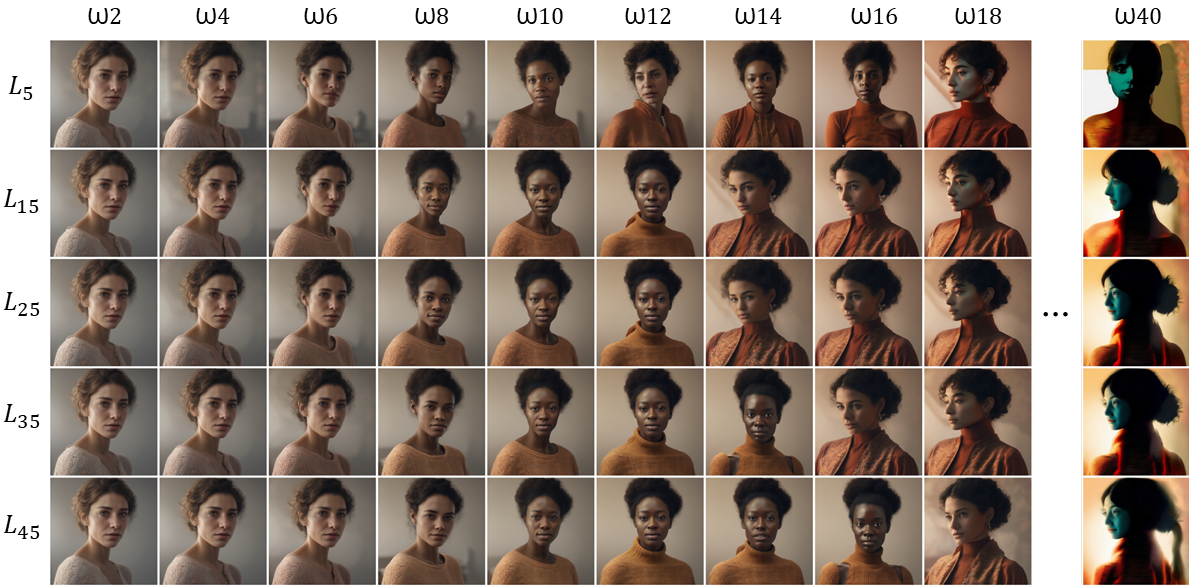
\includegraphics[width=1\linewidth]{images/weight_latent_transition.png}

   \caption{\textbf{Comparison of results with $d_{Z}$ trained at different latents $L$ and applied at different weights $\omega$.} Generations of the same woman in its transition to dark skin.}
   \label{fig:gallery_black_woman}
\end{figure}

\footnotetext{Presence of classes through CLIP's classification: ["A picture of a black [man/woman]", "A picture of a white [man/woman]"], ["A picture of a woman", "A picture of a man"], ["A picture of a Western wedding", "A picture of an Indian wedding"]. A user study is used to evaluate the complex generations (\textit{Wedding}, \textit{African man}) given classification with defined classes in these cases does not match reality.}


%We leverage the discrepancy metric used by \cite{chuang2023debiasing},the L2 norm between empirical and uniform distributions. 

% We use two metrics to quantify distribution diversity and image quality. (1) Distribution Discrepancy (DKL). 


